\documentclass[sigconf,anonymous]{acmart}%%
\usepackage{graphicx}
\usepackage{amsmath}
\usepackage{algorithmic}
\usepackage{textcomp}
\usepackage{booktabs}
\usepackage{multirow}
\usepackage{xcolor}
\usepackage{subcaption}
\usepackage{array}
\usepackage{ragged2e}
\usepackage{tikz}
\usepackage{comment}
\usetikzlibrary{positioning, arrows.meta, fit, backgrounds, calc, shapes.geometric}
\newcolumntype{P}[1]{>{\RaggedRight\arraybackslash}p{#1}}
\hypersetup{colorlinks=true, allcolors=blue}

\AtBeginDocument{%
  \providecommand\BibTeX{{%
    Bib\TeX}}}

\setcopyright{none}
\settopmatter{printacmref=false}

\begin{document}

\title{Maritime Spatio-Temporal Graph Network for Vessel ETA Prediction: An Empirical Study on Trans-Pacific Routes}

\author{Anonymous}
\affiliation{%
  \institution{Anonymous Institution}
  \city{Anonymous City}
  \country{Anonymous Country}}
\email{anonymous@example.com}

\renewcommand{\shortauthors}{Anonymous}

\begin{abstract}
Accurate Estimated Time of Arrival (ETA) prediction for ocean-going vessels is critical for port logistics, berth scheduling, and supply chain management.
While numerous deep learning architectures have been proposed for time-series forecasting, their relative effectiveness for maritime ETA remains unclear.
In this paper, we present two contributions.
First, we conduct a systematic empirical comparison of ten forecasting models spanning five architectural families---recurrent (LSTM, GRU), convolutional (1D-CNN, TCN), attention-based (Transformer, Conv-Transformer, Informer), tree-based (XGBoost), and feedforward (MLP, Ridge)---on a large-scale trans-Pacific AIS dataset comprising 35.9 million position reports and 9,087 voyages.
Second, we propose MSTGN (Maritime Spatio-Temporal Graph Network), which constructs a route graph based on ocean grid cells and uses Graph Convolutional Networks (GCN) to learn spatial context for ETA prediction.
Our results reveal that while XGBoost achieves strong single-model performance (MAE = 15.14\,h), our proposed MSTGN with enriched statistical features and GCN-derived spatial embeddings achieves competitive single-model accuracy (MAE = 15.13\,h) through ensemble knowledge distillation, surpassing XGBoost without requiring multiple inference-time models.
Ablation studies show that statistical feature engineering is the dominant factor in prediction quality, that MSTGN functions as a graph-augmented feature fusion model (rather than an end-to-end spatio-temporal network), and that knowledge distillation from a multi-seed ensemble effectively transfers collective knowledge into a single compact model.
Beyond point-prediction accuracy, we apply ensemble-based conformal prediction to produce calibrated prediction intervals with finite-sample coverage guarantees, achieving 90\% coverage with adaptive intervals of 64.3\,h mean width.
We propose Duration-Stratified Calibration Error (DSCE), a metric for assessing interval reliability across voyage duration strata, and derive operationally actionable buffer times for port scheduling.
These findings reveal that for single-step vessel ETA prediction, compact statistical features combined with spatial graph context, knowledge distillation, and conformal uncertainty quantification provide an effective and operationally practical approach.
\end{abstract}


\keywords{vessel ETA prediction, maritime forecasting, AIS data, graph neural networks, knowledge distillation, conformal prediction, uncertainty quantification}

\maketitle

\section{Introduction}

Vessel Estimated Time of Arrival (ETA) prediction is a fundamental task in maritime logistics.
Accurate ETAs enable port operators to optimize berth allocation, coordinate crane assignments, and reduce vessel waiting times, with significant economic and environmental implications~\cite{unctad2023}.
The proliferation of Automatic Identification System (AIS) data---broadcasting vessel position, speed, and course at frequent intervals---has created an opportunity for data-driven approaches to ETA prediction~\cite{fang2022}.

A wide range of machine learning methods have been applied to this problem.
Recurrent neural networks such as LSTM~\cite{zhang2022lstm} and GRU~\cite{han2021gru} naturally model the sequential nature of vessel trajectories.
Convolutional approaches, including Temporal Convolutional Networks (TCN)~\cite{bai2018tcn}, capture local temporal patterns through dilated causal convolutions.
Transformer-based architectures~\cite{dong2023transformer, zhou2021informer} leverage self-attention to model long-range dependencies.
Meanwhile, gradient-boosted tree methods like XGBoost~\cite{chen2016xgboost} remain competitive through hand-crafted feature engineering.

Despite this diversity of approaches, a systematic comparison under controlled conditions is still lacking.
Most existing studies evaluate only one or two architectures, use different datasets with inconsistent preprocessing pipelines, and often omit critical experimental details---making cross-study comparisons unreliable.
Recent comprehensive surveys in time-series forecasting~\cite{kim2025comprehensive, zeng2023transformers} have emphasized the importance of fair benchmarking, revealing that simpler models often rival or surpass complex architectures when evaluated properly.

% Identify the gap
This paper addresses this gap by conducting a rigorous empirical comparison of ten forecasting models from five architectural families on a large-scale trans-Pacific AIS dataset.
Our model selection follows the taxonomy proposed in recent deep time-series forecasting surveys~\cite{kim2025comprehensive}: we include at least one representative from each major family (recurrent, convolutional, attention-based, tree-based, and feedforward) to ensure comprehensive coverage.
All models are trained and evaluated under identical conditions---including data splits, feature sets, normalization, loss function, optimizer, and early-stopping criteria---to isolate the effect of model architecture.

Our main contributions are:
\begin{enumerate}
    \item A fair, large-scale empirical comparison of ten models spanning five architectural families for vessel ETA prediction, providing controlled benchmarks for maritime forecasting.
    \item A novel Maritime Spatio-Temporal Graph Network (MSTGN) that constructs a route graph over ocean grid cells and fuses GCN-derived spatial context with enriched statistical features, achieving competitive single-model performance through knowledge distillation (MAE = 15.13\,h), surpassing XGBoost (15.14\,h) without ensemble inference.
    \item An ensemble knowledge distillation framework that trains a multi-seed teacher ensemble (15 models, top-7 achieving MAE = 14.95\,h) and distills its knowledge into a single student model that retains virtually all of the ensemble's advantage.
    \item Ablation studies demonstrating that (a) statistical feature engineering is the dominant factor, (b) temporal sequence modeling adds limited value, (c) incorporating meteorological features yields a 7.1\% MAE improvement, (d) MSTGN is best understood as a graph-augmented statistical fusion model rather than an end-to-end spatio-temporal network, and (e) the $2^\circ{\times}2^\circ$ grid resolution is empirically validated against $1^\circ$ and $4^\circ$ alternatives.
    \item A large-deviation analysis identifying that 96\% of extreme prediction errors ($>$100\,h) are systematic underestimates concentrated in ultra-long voyages, with evaluation of remediation strategies achieving up to 5\% relative tail error reduction.
    \item An uncertainty quantification framework using ensemble-based conformal prediction that produces calibrated prediction intervals, together with a novel Duration-Stratified Calibration Error (DSCE) metric and operationally actionable buffer time recommendations for port scheduling.
\end{enumerate}

\section{Related Work}
ETA prediction research falls into two branches: path/trajectory-based methods and machine-learning feature-engineering methods~\cite{leiPredictingVesselArrival2024}. AIS data provides diverse dynamic attributes (location, heading, speed) and static vessel details~\cite{yangHarnessingPowerMachine2024}. In the following subsections we review representative studies from each category.

\subsection{ETA Prediction Based on Path Finding}
Path-based methods preserve explicit spatial structure rather than treating ETA as tabular regression. Park et al.~\cite{parkVesselEstimatedTime2021} combined AIS route grids, Q-learning path search, and MCMC speed sampling to stabilize long-distance predictions. Yoon et al.~\cite{yoonEnhancingContainerVessel2023} built representative historical routes from prior port calls to map real-time AIS positions for ETA at Busan New Port. As reviewed by Jiang et al.~\cite{jiangPredictionVesselArrival2025}, such approaches are most effective when route structure is highly regular.

\subsection{ETA Prediction Based on Feature Engineering}
Feature-engineering methods treat ETA as supervised regression over AIS variables and operational covariates. Yu et al.~\cite{yuShipArrivalPrediction2018} showed that RF models link ETA forecasts directly to berth scheduling decisions. The branch has since evolved toward multi-source fusion and stacking: Kolley et al.~\cite{kolleyRobustBerthScheduling2022} integrated machine-learned ETA into robust berth scheduling; Lei et al.~\cite{leiPredictingVesselArrival2024} incorporated inland waterway factors via tree-based stacking; Chu et al.~\cite{chuVesselArrivalTime2025} fused port call records with AIS for improved accuracy; and Saber et al.~\cite{saberHighaccuracyPredictionVessels2025} achieved strong results with a hybrid Extra Trees/LightGBM stack. These studies confirm that operational and environmental covariates are increasingly central to model design.

\subsection{Research Gaps in Existing ETA Prediction Studies}
The literature shows clear progress but lacks a unified benchmark comparing model families for full-voyage open-ocean ETA prediction~\cite{jiangPredictionVesselArrival2025,nomanReviewVesselTime2025}. Existing studies are fragmented across port areas, inland waterways, and near-arrival settings, making it unclear whether gains come from model architecture or experimental design differences. These gaps motivate the present study, which evaluates ten models under a unified protocol to clarify which modeling ingredients are genuinely useful for long trans-Pacific voyages.

\section{Methodology}

\subsection{Problem Formulation}

Given a vessel's historical AIS trajectory $\mathbf{X} = \{x_1, x_2, \ldots, x_T\}$, where each observation $x_t \in \mathbb{R}^{d}$ contains $d$-dimensional navigation and meteorological features at time step $t$, the objective is to predict the remaining sailing time $\hat{y} \in \mathbb{R}^{+}$ to the end of the current voyage segment---i.e., the time until the vessel completes its active open-sea transit and arrives at its next port of call.
We focus exclusively on the in-transit sailing phase, where the vessel's dynamics are governed by speed, heading, ocean currents, and weather conditions. Port-dwell time (berth waiting, cargo handling, customs processing) is excluded from the prediction target because it depends on logistical factors that are unobservable from AIS data alone.



\subsection{Data Preparation and System Overview}
\label{sec:voyage_extraction}
The overall pipeline is illustrated in Fig.~\ref{fig:architecture}. Raw AIS records are first cleaned, segmented into voyages, matched with meteorological observations, and organized into fixed-length input sequences. The processed sequences are then fed into one of the candidate forecasting models to predict the remaining sailing time.

\begin{enumerate}
    \item \textbf{Data Preprocessing}: Raw AIS records are cleaned, segmented into individual voyages via speed-based port-stop detection, augmented with meteorological features, and organized into fixed-length input sequences.
    \item \textbf{Sailing Time Prediction}: One of ten candidate models processes the input sequences to predict the remaining sailing time for the current voyage segment.
\end{enumerate}

\begin{figure*}[t]
\centering
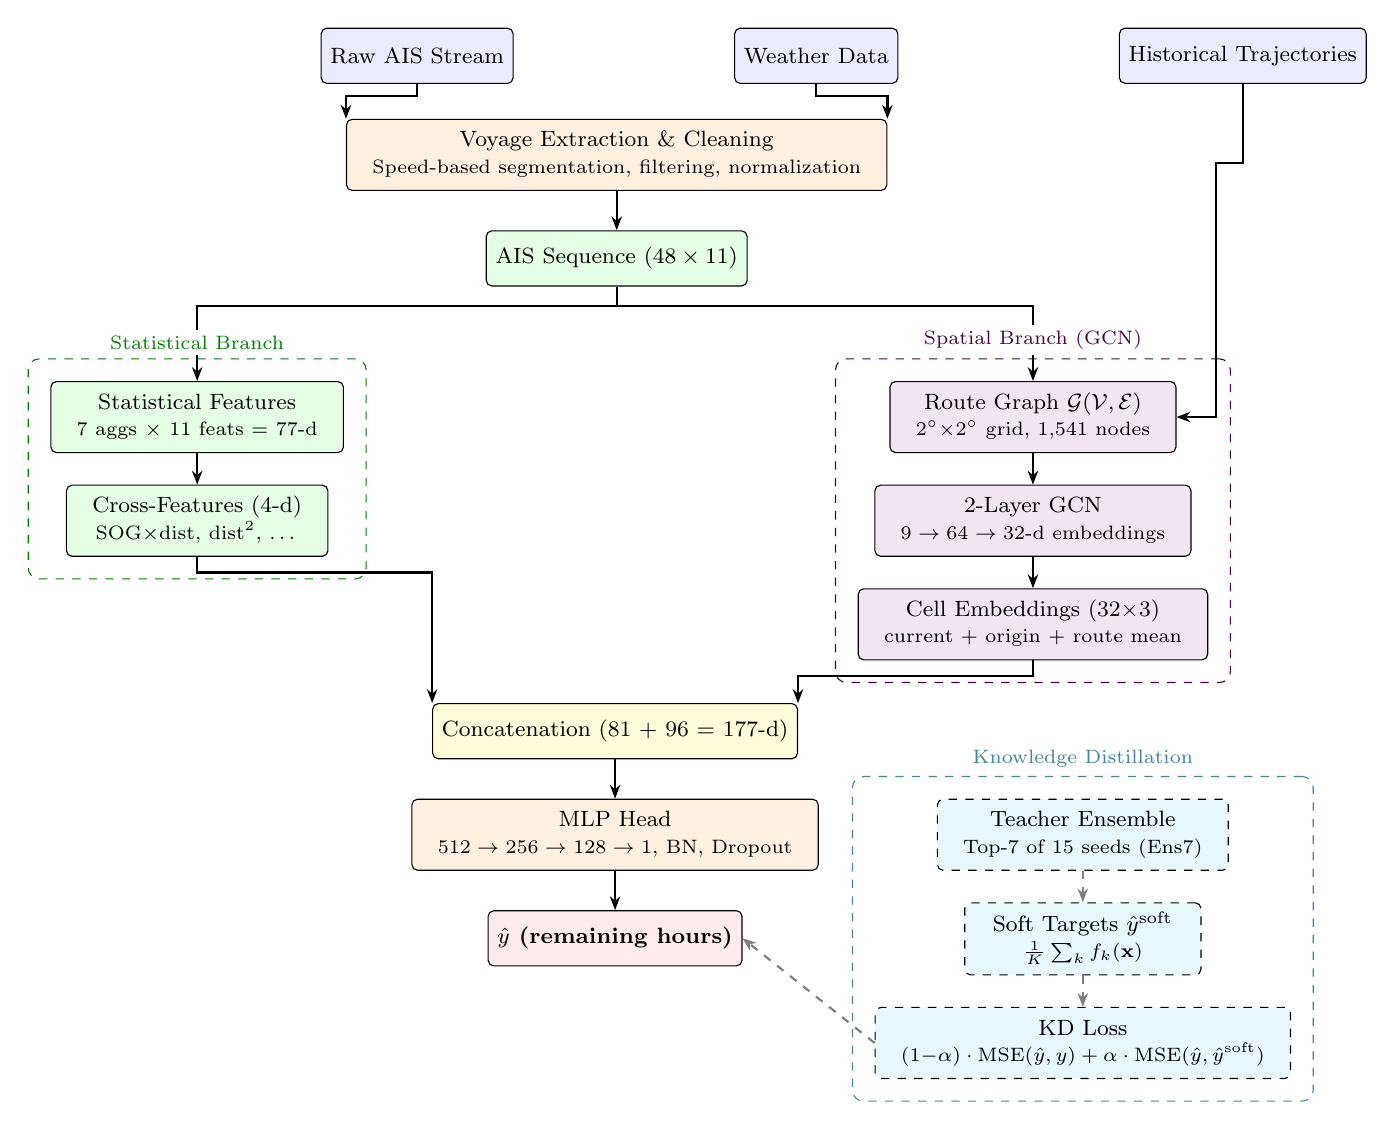
\begin{tikzpicture}[
    node distance=0.5cm and 0.6cm,
    box/.style={draw, rounded corners=2pt, minimum height=0.7cm, text centered, font=\footnotesize},
    data/.style={box, fill=blue!8, minimum width=2.0cm},
    proc/.style={box, fill=orange!12, minimum width=2.4cm},
    feat/.style={box, fill=green!10, minimum width=2.4cm},
    graph/.style={box, fill=violet!10, minimum width=2.4cm},
    fuse/.style={box, fill=yellow!15, minimum width=2.4cm},
    outnode/.style={box, fill=red!8, minimum width=1.8cm, font=\footnotesize\bfseries},
    kd/.style={box, fill=cyan!10, minimum width=2.4cm, dashed},
    arr/.style={-{Stealth[length=5pt]}, thick},
    darr/.style={-{Stealth[length=5pt]}, thick, dashed, gray},
    lbl/.style={font=\scriptsize, text=black!70},
]

% === Row 0: Data sources ===
\node[data] (ais) {Raw AIS Stream};
\node[data, right=2.8cm of ais] (wx) {Weather Data};
\node[data, right=2.8cm of wx] (graph_data) {Historical Trajectories};

% === Row 1: Preprocessing ===
\node[proc, below=0.8cm of $(ais)!0.5!(wx)$] (preproc) {\begin{tabular}{c}Voyage Extraction \& Cleaning\\\scriptsize Speed-based segmentation, filtering, normalization\end{tabular}};

% === Row 2: Sequence output ===
\node[feat, below=0.5cm of preproc, minimum width=3.2cm] (seq) {AIS Sequence ($48 \times 11$)};

% Arrows: data 鈫?preproc
\draw[arr] (ais.south) -- ++(0,-0.15) -| (preproc.north -| preproc.west);
\draw[arr] (wx.south) -- ++(0,-0.15) -| (preproc.north -| preproc.east);

\draw[arr] (preproc) -- (seq);

% === Row 3: Two branches ===
% Left: Statistical branch
\node[feat, below left=1.2cm and 1.8cm of seq] (stat) {\begin{tabular}{c}Statistical Features\\\scriptsize 7 aggs $\times$ 11 feats = 77-d\end{tabular}};
\node[feat, below=0.4cm of stat] (cross) {\begin{tabular}{c}Cross-Features (4-d)\\\scriptsize SOG$\times$dist, dist$^2$, \ldots\end{tabular}};

% Right: Graph branch
\node[graph, below right=1.2cm and 1.8cm of seq] (rgraph) {\begin{tabular}{c}Route Graph $\mathcal{G}(\mathcal{V}, \mathcal{E})$\\\scriptsize $2^\circ{\times}2^\circ$ grid, 1,541 nodes\end{tabular}};
\node[graph, below=0.4cm of rgraph] (gcn) {\begin{tabular}{c}2-Layer GCN\\\scriptsize $9 \to 64 \to 32$-d embeddings\end{tabular}};
\node[graph, below=0.4cm of gcn] (cell_emb) {\begin{tabular}{c}Cell Embeddings ($32{\times}3$)\\\scriptsize current + origin + route mean\end{tabular}};

% Arrows for branches
\draw[arr] (seq.south) -- ++(0,-0.25) -| (stat.north);
\draw[arr] (stat) -- (cross);
\draw[arr] (seq.south) -- ++(0,-0.25) -| (rgraph.north);
\draw[arr] (graph_data.south) -- ++(0,-1.0) -| ([xshift=0.5cm]rgraph.east) -- (rgraph.east);
\draw[arr] (rgraph) -- (gcn);
\draw[arr] (gcn) -- (cell_emb);

% === Row 4: Fusion ===
\node[fuse, below=1.2cm of $(cross.south)!0.5!(cell_emb.south)$, minimum width=3.0cm] (concat) {Concatenation (81 + 96 = 177-d)};

\draw[arr] (cross.south) -- ++(0,-0.2) -| (concat.north -| concat.west);
\draw[arr] (cell_emb.south) -- ++(0,-0.2) -| (concat.north -| concat.east);

% === Row 5: MLP Head ===
\node[proc, below=0.5cm of concat] (mlp) {\begin{tabular}{c}MLP Head\\\scriptsize $512 \to 256 \to 128 \to 1$, BN, Dropout\end{tabular}};
\draw[arr] (concat) -- (mlp);

% === Row 6: Output ===
\node[outnode, below=0.5cm of mlp] (yhat) {$\hat{y}$ (remaining hours)};
\draw[arr] (mlp) -- (yhat);

% === KD box (right side) ===
\node[kd, right=1.5cm of mlp, minimum width=3.0cm] (ens) {\begin{tabular}{c}Teacher Ensemble\\\scriptsize Top-7 of 15 seeds (Ens7)\end{tabular}};
\node[kd, below=0.4cm of ens, minimum width=3.0cm] (soft) {\begin{tabular}{c}Soft Targets $\hat{y}^{\text{soft}}$\\\scriptsize $\frac{1}{K}\sum_k f_k(\mathbf{x})$\end{tabular}};
\node[kd, below=0.4cm of soft, minimum width=3.0cm] (kdloss) {\begin{tabular}{c}KD Loss\\\scriptsize $(1{-}\alpha)\cdot\text{MSE}(\hat{y},y) + \alpha\cdot\text{MSE}(\hat{y},\hat{y}^{\text{soft}})$\end{tabular}};

\draw[darr] (ens) -- (soft);
\draw[darr] (soft) -- (kdloss);
\draw[darr] (kdloss.west) -- (yhat.east);

% === Background boxes ===
\begin{scope}[on background layer]
    \node[draw=green!50!black, dashed, rounded corners=4pt, inner sep=8pt,
          fit=(stat)(cross)] (stat_box) {};
    \node[draw=violet!60!black, dashed, rounded corners=4pt, inner sep=8pt,
          fit=(rgraph)(gcn)(cell_emb)] (graph_box) {};
    \node[draw=cyan!60!black, dashed, rounded corners=4pt, inner sep=8pt,
          fit=(ens)(soft)(kdloss)] (kd_box) {};
\end{scope}
% Labels above boxes
\node[font=\scriptsize, text=green!50!black, above=1pt of stat_box.north, fill=white, inner sep=2pt] {Statistical Branch};
\node[font=\scriptsize, text=violet!60!black, above=1pt of graph_box.north, fill=white, inner sep=2pt] {Spatial Branch (GCN)};
\node[font=\scriptsize, text=cyan!60!black, above=1pt of kd_box.north, fill=white, inner sep=2pt] {Knowledge Distillation};

\end{tikzpicture}
\caption{Architecture of the proposed MSTGN-KD system. Raw AIS and weather data are preprocessed into 48-step sequences. The statistical branch extracts 81 aggregated features plus 4 cross-features; the spatial branch constructs a route graph and produces GCN cell embeddings. Both are fused and fed through an MLP head. During training, an ensemble teacher provides soft targets via knowledge distillation (dashed lines).}
\label{fig:architecture}
\end{figure*}

Each input sequence consists of $L_{\text{enc}} = 48$ consecutive AIS observations. At each time step $t$, the feature vector $x_t \in \mathbb{R}^{11}$ includes:
\begin{itemize}
    \item \textbf{Navigation features} ($d_{\text{nav}} = 6$): latitude, longitude, speed over ground (SOG), course over ground (COG), great-circle distance to destination ($\text{dist\_km}$), and bearing difference ($\Delta\theta$) between COG and the bearing toward the destination.
    \item \textbf{Meteorological features} ($d_{\text{wx}} = 5$): temperature, wind speed, wind level, mean sea-level pressure (PRMSL), and visibility.
\end{itemize}
Navigation features are min-max normalized to $[0,1]$ with clipping at $[-0.5,1.5]$, and the target variable is log-standardized as $\tilde{y} = (\ln(1+y)-\mu)/\sigma$, where $\mu$ and $\sigma$ are computed from the training set.

Voyages are extracted from the continuous AIS stream using speed-based port-stop detection:
\begin{enumerate}
    \item \textbf{Stop detection}: a vessel is classified as stopped when its SOG falls below $\tau_{\text{stop}} = 0.3$~knots.
    \item \textbf{Stop validation}: a stopped segment is treated as a valid port stop only if its duration exceeds $T_{\text{min\_stop}} = 2$~hours.
    \item \textbf{Sailing segment filtering}: sailing segments between successive port stops are retained only if duration $\geq T_{\text{min\_sail}} = 6$~hours and the number of AIS records $\geq N_{\text{min}} = 50$.
    \item \textbf{Route filtering}: we retain only voyages connecting Asian ports (longitude $> 100^\circ$E or $< 150^\circ$W) to U.S.\ West Coast ports ($-130^\circ < \text{lon} < -115^\circ$).
    \item \textbf{Duration filtering}: voyages exceeding 720 hours are excluded as likely erroneous or multi-stop itineraries.
\end{enumerate}
This procedure yields 9,087 valid voyages from 3,940 unique vessels.

\subsection{Benchmarked Models}
\label{sec:model_selection}
Following recent deep time-series forecasting surveys~\cite{kim2025comprehensive, zeng2023transformers}, we evaluate ten models spanning five major families:
\begin{enumerate}
    \item \textbf{Recurrent models}: \textit{LSTM}~\cite{hochreiter1997lstm} and \textit{GRU}~\cite{cho2014gru}.
    \item \textbf{Convolutional models}: \textit{1D-CNN} and \textit{TCN}~\cite{bai2018tcn}.
    \item \textbf{Attention-based models}: \textit{Transformer}~\cite{vaswani2017attention}, \textit{Conv-Transformer}, and \textit{Informer}~\cite{zhou2021informer}.
    \item \textbf{Tree-based model}: \textit{XGBoost}~\cite{chen2016xgboost}.
    \item \textbf{Feedforward baselines}: \textit{MLP} and \textit{Ridge Regression}.
\end{enumerate}

All neural models use the same $48 \times 11$ sequence input, whereas XGBoost and Ridge operate on hand-crafted tabular features. Table~\ref{tab:model_configs} summarizes the main configurations and parameter counts.

\begin{table}[t]
    \centering
    \caption{Model Configurations and Parameter Counts}
    \label{tab:model_configs}
    \begin{tabular}{llr}
        \toprule
        \textbf{Model} & \textbf{Key Configuration} & \textbf{Params} \\
        \midrule
        Ridge & $L_2$ regularization & -- \\
        MLP & $512{\to}256{\to}128$, BN, dropout & 270K \\
        XGBoost & 500 rounds, GPU hist & -- \\
        \midrule
        LSTM & 2 layers, $h{=}256$ & 802K \\
        GRU & 2 layers, $h{=}256$ & 610K \\
        \midrule
        1D-CNN & 3 Conv1d, MaxPool, AvgPool & 350K \\
        TCN & 4 dilated blocks $[128,128,256,256]$ & 600K \\
        \midrule
        Transformer & 3 enc layers, $d{=}256$, 8 heads & 1.6M \\
        Conv-Trans. & 2 Conv1d $+$ 2 enc layers, $d{=}256$ & 1.5M \\
        Informer & 2 enc $+$ 1 dec, $d{=}512$, ProbSparse & 11.3M \\
        \midrule
        MSTGN-MLP & Stats(44) + 2-layer GCN, $d_\text{cell}{=}32$ & 238K \\
        MSTGN-MLP2 & Stats(81) + 2-layer GCN + cross-feats & 273K \\
        MSTGN-Late & GRU + GCN late fusion & 737K \\
        StatMLP & Stats 44-dim, $256{\to}128{\to}64$ & 189K \\
        \bottomrule
    \end{tabular}
\end{table}

Among the evaluated attention models, Informer follows the original ProbSparse-attention and distilling design~\cite{zhou2021informer}. Since it serves as a baseline rather than the main proposed method, we omit further architectural detail here.


\subsection{Maritime Route Graph and MSTGN}
\label{sec:mstgn}

To explicitly encode spatial dependencies in vessel movements, we derive a maritime route graph $\mathcal{G} = (\mathcal{V}, \mathcal{E})$ from historical AIS trajectories and use it as the underlying spatial structure of MSTGN.

\paragraph{Route graph construction.}
The ocean surface is discretized into $2^\circ \times 2^\circ$ grid cells, and a cell is retained as a node if it contains at least 50 AIS observations, yielding $|\mathcal{V}| = 1{,}541$ active nodes plus one \textit{unknown} node for rare out-of-distribution cells. Edges are defined from two sources:
\begin{itemize}
    \item \textbf{Transition edges}: directed edges between consecutively visited cells, weighted by log-transformed transition counts.
    \item \textbf{Geographic edges}: undirected edges between border-sharing cells.
\end{itemize}
The resulting graph contains 4{,}772 transition edges and 2{,}110 geographic edges (13{,}033 non-zero entries in the symmetrized adjacency matrix). Each node is assigned a 9-dimensional feature vector comprising mean SOG, SOG standard deviation, mean temperature, mean wind speed, mean pressure, mean visibility, log vessel count, and normalized center coordinates.
\paragraph{MSTGN architecture.}
MSTGN is designed as a graph-augmented feature-fusion model rather than an end-to-end spatio-temporal graph network. In the spatial branch, a two-layer GCN~\cite{kipf2017gcn} produces 32-dimensional cell embeddings:
\begin{equation}
    \mathbf{H}^{(l+1)} = \sigma\!\left(\hat{\mathbf{A}} \, \mathbf{H}^{(l)} \mathbf{W}^{(l)} + \mathbf{b}^{(l)}\right),
\end{equation}
where $\hat{\mathbf{A}} = \tilde{\mathbf{D}}^{-1/2}\tilde{\mathbf{A}}\tilde{\mathbf{D}}^{-1/2}$ and $\sigma$ is ReLU. For each input sequence, the embedding of the last-step grid cell is retrieved as spatial context for prediction.

In parallel, the non-graph branch uses one of two alternatives:
\begin{itemize}
    \item \textbf{GRU encoder}: a 2-layer GRU with attention pooling over hidden states.
    \item \textbf{Statistical features}: hand-crafted summaries extracted from the 48-step input window.
\end{itemize}
The spatial embedding is concatenated with the temporal or statistical representation and fed to an MLP prediction head.

\paragraph{Model variants.}
We evaluate five MSTGN variants:
\begin{itemize}
    \item \textbf{MSTGN-MLP}: 44-dimensional statistical features + GCN cell embeddings.
    \item \textbf{MSTGN-MLP2}: enriched statistical features + cross-features + multiple graph contexts.
    \item \textbf{MSTGN-LateFusion}: GRU encoder with GCN embedding fused at the output layer.
    \item \textbf{StatMLP}: statistical features only.
    \item \textbf{MSTGN-GRU}: GRU with cell embeddings concatenated to every timestep.
\end{itemize}

For MSTGN-MLP2 the branch is expanded to 81 dimensions: 7 aggregations (last-step, mean, std, diff, min, max, recent-12-step mean) $\times$ 11 features, plus 4 cross-features ($\text{SOG}{\times}\text{dist}$, $\text{dist}^2$, $\text{SOG}{\times}\Delta\theta$, $\Delta\text{SOG}{\times}\text{dist}$) and 3 graph contexts (current-cell, origin-cell, mean-route embeddings). The fused representation is processed by a $512 \to 256 \to 128 \to 1$ MLP head with BatchNorm and 10\% dropout.

\paragraph{Ensemble and knowledge distillation.}
To exploit training stochasticity, we train 15 MSTGN-MLP2 models with different random seeds and form an ensemble by averaging the top-$K$ models selected by validation loss:
\begin{equation}
    \hat{y}_{\text{ens}} = \frac{1}{K} \sum_{k=1}^{K} \hat{y}^{(k)}.
\end{equation}
We report results for $K \in \{5,7,15\}$, and the top-7 ensemble achieves the best MAE. To avoid multi-model inference at deployment, we further apply ensemble knowledge distillation~\cite{hinton2015distilling} and train the student model with
\begin{equation}
    \mathcal{L} = (1-\alpha)\cdot\mathcal{L}_{\text{MSE}}(\hat{y}, y) + \alpha\cdot\mathcal{L}_{\text{MSE}}(\hat{y}, \hat{y}^{\text{soft}}),
    \label{eq:kd_loss}
\end{equation}
where $\hat{y}^{\text{soft}}$ denotes the teacher ensemble prediction. We find that $\alpha = 0.6$ yields the best result (Table~\ref{tab:kd_ablation}).


%==============================================================
\section{Experiments}
%==============================================================

\subsection{Experimental Setup}

We evaluate all methods on a proprietary AIS dataset covering trans-Pacific shipping routes between Chinese ports and the U.S.\ West Coast from January 2021 to March 2025. The raw data contain 35.9 million AIS records from 3,940 vessels. Each record includes MMSI, timestamp, longitude, latitude, speed over ground (SOG), and course over ground (COG); we additionally match temperature, wind speed, wind level (Beaufort scale), mean sea-level pressure, and horizontal visibility from contemporary weather data sources. Voyages are extracted using the procedure in Section~\ref{sec:voyage_extraction}, yielding 9,087 valid voyages and 13.1M/2.9M/2.9M train/validation/test sequences under a 70/15/15 split. All models use the same 48-step input with 11 features per time step.

All models are evaluated under identical conditions: the same voyage-level split, the same 11-dimensional feature set, the same min-max normalization with log-standardized targets, Huber loss ($\delta = 1.0$), and batch size 4,096. Neural models are trained with Adam at $\mathrm{lr}=10^{-3}$ and patience-3 early stopping; Informer follows its original training recipe with $\mathrm{lr}=4\times 10^{-4}$ and ReduceLROnPlateau. Experiments are run on a single NVIDIA RTX PRO 6000 GPU (96\,GB VRAM), and XGBoost uses GPU histogram training. Data loading uses NumPy memmap, 64 workers, and pinned memory to handle the 13M+ training sequences.

We report MAE, RMSE, MAPE ($y_i{>}24$\,h only to avoid near-arrival artifacts), MedAE, $R^2$, and Within-$\tau$ accuracy for $\tau{\in}\{6,12,24\}$\,h. For uncertainty analysis (Section~\ref{sec:uq}) we additionally report PICP, MPIW, and DSCE.


\subsection{Main Results}

Table~\ref{tab:main_results} reports the test-set results for all methods.

\begin{table}[t]
    \centering
    \caption{Comparison of ETA Prediction Methods on Test Set. All models use standard Huber loss except MSTGN-MLP2 and MSTGN-KD which use MSE. Best results in \textbf{bold}, second-best \underline{underlined}.}
    \label{tab:main_results}
    \setlength{\tabcolsep}{4pt}
    \begin{tabular}{llccc}
        \toprule
        \textbf{Family} & \textbf{Method} & \textbf{MAE (h)} & \textbf{RMSE (h)} & \textbf{MAPE (\%)} \\
        \midrule
        \multirow{2}{*}{Feedforward} & Ridge & 58.30 & 367.19 & 29.35 \\
        & MLP & 15.73 & 26.80 & 9.67 \\
        \midrule
        \multirow{2}{*}{Recurrent} & LSTM & 15.79 & 27.40 & 9.43 \\
        & GRU & 16.03 & 27.28 & 9.62 \\
        \midrule
        \multirow{2}{*}{Convolutional} & 1D-CNN & 16.08 & 27.53 & 9.90 \\
        & TCN & 17.19 & 28.13 & 10.95 \\
        \midrule
        Tree & XGBoost & 15.14 & \textbf{26.05} & 9.33 \\
        \midrule
        \multirow{3}{*}{Attention} & Transformer & 18.12 & 29.78 & 10.67 \\
        & Conv-Trans. & 16.60 & 27.52 & 10.07 \\
        & Informer & 16.20 & 27.26 & 10.53 \\
        \midrule
        \multirow{7}{*}{Graph} & MSTGN-MLP & 15.40 & 26.57 & 9.50 \\
        & StatMLP & 15.41 & 27.08 & 9.43 \\
        & MSTGN-Late & 15.56 & 26.74 & 9.68 \\
        & MSTGN-MLP2 & 15.28 & 26.58 & 9.33 \\
        & MSTGN-Ens7 & \textbf{14.95} & \underline{26.08} & \textbf{9.16} \\
        & \underline{MSTGN-KD} & \underline{15.13} & 26.16 & \underline{9.33} \\
        \bottomrule
    \end{tabular}
\end{table}

MSTGN-Ens7 achieves the best overall accuracy (MAE 14.95\,h), while MSTGN-KD achieves the best single-model performance (15.13\,h), narrowly surpassing XGBoost (15.14\,h). Knowledge distillation transfers 89\% of the ensemble gain ($15.28 \to 15.13$\,h) into a single 273K-parameter model. The gain is not solely due to distillation: MSTGN-MLP2 already improves over MSTGN-MLP (15.28 vs.\ 15.40\,h), indicating that enriched statistical features close most of the gap before compression.

The broader ranking is equally informative. Statistical-feature models outperform sequence-heavy alternatives: StatMLP (15.41\,h) matches MSTGN-MLP within 0.01\,h, whereas GRU-based models remain about 0.6\,h worse. Attention-based models also provide little benefit in this setting: Transformer performs worst among the neural baselines (18.12\,h), and both Informer (16.20\,h) and Conv-Transformer (16.60\,h) trail the much smaller MLP (15.73\,h). These results suggest that, for single-step ETA regression, compact feature summaries are more effective than complex temporal encoders.

Graph structure yields modest but consistent gains. Adding GCN cell embeddings slightly improves both the statistical branch (MSTGN-MLP 15.40\,h vs.\ StatMLP 15.41\,h) and the GRU branch (MSTGN-Late 15.56\,h vs.\ GRU 16.03\,h). The magnitude of the gain is small, which suggests that latitude and longitude already encode most positional information, while the graph provides residual route-level context.

Fig.~\ref{fig:analysis} examines the best single model, MSTGN-KD ($\alpha{=}0.6$). Predictions align closely with ground truth across most of the range, but MAE rises steadily with remaining voyage time: it is below 3\,h within the first day and exceeds 25\,h beyond 14 days. The error distribution is approximately symmetric with a slight negative bias (mean $=-2.56$\,h, median $=+1.18$\,h). The cumulative accuracy curve shows that 50\% of predictions fall within 8.3\,h, 90\% within 35.2\,h, and 95\% within 51.4\,h. Beyond MAE, MSTGN-KD achieves MedAE $= 8.31$\,h, $R^2 = 0.958$, and 41.1\% within $\pm6$\,h; the ensemble further improves MedAE to 8.09\,h and Within-24h accuracy to 82.1\%.

\begin{figure*}[t]
    \centering
    \includegraphics[width=\textwidth]{analysis_plots.pdf}
    \caption{Prediction quality analysis of the best single model (MSTGN-KD, $\alpha{=}0.6$, MAE~$=$~15.13\,h) on the test set (2.86M samples). (a)~Predicted vs.\ actual remaining time (hexbin density); (b)~MAE stratified by true remaining voyage time; (c)~error distribution histogram; (d)~cumulative fraction of predictions within a given absolute error threshold.}
    \label{fig:analysis}
\end{figure*}
Table~\ref{tab:lit_comparison} is a positioning table, not a direct numerical comparison---routes, target definitions, and protocols differ substantially. Most prior studies focus on port areas or near-arrival prediction; even Lloret-Batlle et al.~\cite{lloretbatlle2025} cover only the final $\sim$1{,}500~NM of the trans-Pacific leg. Our full-voyage setting begins at voyage start ($>$5{,}000~NM from port), so a larger absolute MAE is expected.


\begin{table*}[t]
    \centering
    \caption{Recent maritime ETA prediction studies. ``Dist.''~denotes the approximate sailing distance covered by the dataset. Metrics are as reported by the original authors and are \textbf{not directly comparable} due to differences in route type, prediction granularity, and evaluation protocol.}
    \label{tab:lit_comparison}
   % \footnotesize
    \setlength{\tabcolsep}{3pt}
    \renewcommand{\arraystretch}{1.15}
    \begin{tabular}{P{2.5cm} P{1.5cm} P{1.7cm} P{1.5cm} P{1.2cm} P{2.0cm} P{3.8cm}}
        \toprule
        \textbf{Study} & \textbf{Route type} & \textbf{Dist.\ (NM)} & \textbf{Voyages} & \textbf{Models} & \textbf{Best method} & \textbf{Reported result} \\
        \midrule
        Yu et al.~\cite{yuShipArrivalPrediction2018} & Port call & Short & --- & 3 & RF & Classification-based ETA \\
        Kolley et al.~\cite{kolleyRobustBerthScheduling2022} & European port & Short & --- & 4 & KNN & Berth scheduling integration \\
        El~Mekkaoui et al.~\cite{elmekkaouiDeepLearningModels2022} & Bulk port & Short--Med. & --- & 4 & LSTM & First bulk-port DL benchmark \\
        Du et al.~\cite{duSegmentedETAPrediction2025} & Pilotage area & Short & --- & 4 & TCN & Segmented CNN-LSTM method \\
        Lei et al.~\cite{leiPredictingVesselArrival2024} & Inland waterway & Short & --- & 4 & LightGBM & Tree-based stacking \\
        Saber et al.~\cite{saberHighaccuracyPredictionVessels2025} & Seaport & Med. & --- & 4+ & ET+LGB stack & Hybrid stacking, high accuracy \\
        Chu et al.~\cite{chuVesselArrivalTime2025} & Multi-port & Med. & --- & 5+ & Stacked ens. & Port call + AIS fusion \\
        Lloret-Batlle et al.~\cite{lloretbatlle2025} & Cross-Pacific & ${\sim}5{,}500$ & --- & 1 & ANN & MAE $\approx$ 4\,h at 1{,}500\,NM from port \\
        \midrule
        \textbf{This work} & \textbf{Cross-Pacific} & $\boldsymbol{\sim}$\textbf{5,500} & \textbf{9,087} & \textbf{16} & \textbf{MSTGN-KD} & \textbf{MAE = 15.13\,h (full voyage)} \\
        \bottomrule
    \end{tabular}
\end{table*}

Our benchmark compares 16 configurations from six model families under a single shared protocol, so gaps in Table~\ref{tab:main_results} are attributable to model design. MSTGN-KD preserves most of the ensemble gain (15.13 vs.\ 14.95\,h) in a single deployable model without multi-model inference.




\subsection{Ablation Studies}
\label{sec:ablations}

Ablation studies are conducted to isolate the contributions of the input feature set, the spatial design of MSTGN, and the distillation procedure used to compress the ensemble. Taken together, these experiments clarify how meteorological variables, graph construction and fusion strategy, and ensemble-to-student transfer affect overall prediction accuracy.

\subsubsection{Effect of Weather Features}

To quantify the contribution of meteorological features, we train the Informer model with identical hyperparameters using only the six navigation features ($d = 6$) versus the full 11-dimensional input ($d = 11$). As shown in Table~\ref{tab:ablation_weather}, incorporating weather features reduces MAE from 17.43 to 16.20\,h, a 7.1\% relative improvement. This indicates that en-route weather conditions provide complementary information beyond what navigation features alone capture.

\begin{table}[t]
    \centering
    \caption{Ablation: Effect of Weather Features (Informer)}
    \label{tab:ablation_weather}
   % \footnotesize
    \begin{tabular}{lccc}
        \toprule
        \textbf{Features} & \textbf{MAE} & $\Delta$\textbf{MAE} & $\Delta$\textbf{MAE} \\
        & \textbf{(h)} & \textbf{(h)} & \textbf{(\%)} \\
        \midrule
        Nav.\ only ($d=6$) & 17.43 & -- & -- \\
        Nav.\ + Weather ($d=11$) & \textbf{16.20} & $-1.23$ & $-7.1\%$ \\
        \bottomrule
    \end{tabular}
\end{table}

\subsubsection{Effect of Asymmetric Loss}

To examine whether explicitly penalizing underestimation improves operationally relevant performance, an \textit{Asymmetric Huber Loss} is introduced in which underestimation is weighted by a factor of $\alpha$ and long-haul voyages can be further upweighted through the target value:
\begin{equation}
    \mathcal{L} = \frac{1}{N} \sum_{i=1}^{N} w_{\text{asym}}^{(i)} \cdot w_{\text{target}}^{(i)} \cdot \mathcal{H}_\delta(e_i)
    \label{eq:loss}
\end{equation}
where $w_{\text{asym}} = \alpha$ if $e_i < 0$ (underestimation), else $1$; and $w_{\text{target}} = 1 + \beta \cdot \text{ReLU}(y_i)$.

Two configurations are considered: (A)~$\alpha{=}1.5, \beta{=}0.3$ and (B)~$\alpha{=}1.2$,\allowbreak $\beta{=}0$. Both degrade accuracy substantially (Table~\ref{tab:ablation_loss}): configuration A increases MAE by 13.8\% (16.20 $\to$ 18.43\,h), and configuration B increases it by 17.6\% (16.20 $\to$ 19.05\,h).

\begin{table}[t]
    \centering
    \caption{Ablation: Asymmetric Loss on Informer (Negative Result)}
    \label{tab:ablation_loss}
    \begin{tabular}{lccc}
        \toprule
        \textbf{Loss Configuration} & \textbf{MAE (h)} & \textbf{RMSE (h)} & \textbf{MAPE (\%)} \\
        \midrule
        Huber (symmetric) & \textbf{16.20} & \textbf{27.26} & 10.53 \\
        Asym. ($\alpha{=}1.5, \beta{=}0.3$) & 18.43 & 30.00 & 12.32 \\
        Asym. ($\alpha{=}1.2, \beta{=}0$) & 19.05 & 33.54 & \textbf{11.13} \\
        \bottomrule
    \end{tabular}
\end{table}

Under the present training setup, the asymmetric objective appears to push the model toward overestimation and poorer calibration rather than better operational behavior. We therefore treat asymmetric loss as a cautionary result, not a default design choice.

\subsubsection{Spatial Structure and Model Design}

To disentangle the contributions of temporal sequence modeling, graph structure, and the statistical feature branch, Table~\ref{tab:ablation_graph} compares the main MSTGN components directly.

\begin{table}[t]
    \centering
    \caption{Ablation: Component Contributions of the MSTGN Architecture. ``Stats'' denotes the 44-dim statistical feature vector; ``GRU'' denotes the 2-layer GRU encoder; ``GCN'' denotes the route graph cell embeddings.}
    \label{tab:ablation_graph}
    \begin{tabular}{lccccc}
        \toprule
        \textbf{Variant} & \textbf{Stats} & \textbf{GRU} & \textbf{GCN} & \textbf{MAE (h)} & \textbf{RMSE (h)} \\
        \midrule
        StatMLP          & $\checkmark$   &              &              & 15.41 & 27.08 \\
        MSTGN-MLP        & $\checkmark$   &              & $\checkmark$ & \textbf{15.40} & \textbf{26.57} \\
        MSTGN-Late       &                & $\checkmark$ & $\checkmark$ & 15.56 & 26.74 \\
        GRU (baseline)   &                & $\checkmark$ &              & 16.03 & 27.28 \\
        MSTGN-GRU        &                & $\checkmark^\dagger$ & $\checkmark$ & 16.06 & 28.44 \\
        \bottomrule
    \end{tabular}
    \vspace{2pt}
    {\footnotesize $\dagger$ Cell embedding concatenated to every timestep.}
\end{table}

The clearest pattern is that compact statistical summaries carry most of the predictive signal. StatMLP (15.41\,h) outperforms GRU (16.03\,h) while using a 44-dimensional vector instead of the raw $48{\times}11$ sequence. GCN embeddings still help, but only modestly: MSTGN-MLP improves StatMLP by 0.01\,h MAE and 0.51\,h RMSE, and MSTGN-Late improves GRU by 0.47\,h MAE. Early fusion moves in the opposite direction, with MSTGN-GRU slightly worse than the plain GRU (16.06 vs.\ 16.03\,h), which suggests that repeating static cell embeddings at every timestep weakens rather than helps the recurrent encoder.

To assess sensitivity to the route-graph resolution, MSTGN-MLP2 (without KD) is trained with three cell sizes: $1^\circ{\times}1^\circ$, $2^\circ{\times}2^\circ$, and $4^\circ{\times}4^\circ$. For each resolution, the route graph is rebuilt and cell assignments are recomputed for all training and test samples. Table~\ref{tab:ablation_grid} reports the resulting comparison.

\begin{table}[t]
    \centering
    \caption{Ablation: Effect of Grid Resolution on MSTGN-MLP2 (no KD). Coarser cells average over larger ocean regions; finer cells are sparser due to the minimum-50-count threshold.}
    \label{tab:ablation_grid}
    \begin{tabular}{lcccc}
        \toprule
        \textbf{Cell size} & \textbf{Nodes} & \textbf{MAE (h)} & \textbf{RMSE (h)} & \textbf{MAPE (\%)} \\
        \midrule
        $1^\circ{\times}1^\circ$ & 4,665 & 15.51 & \textbf{26.24} & 9.90 \\
        $2^\circ{\times}2^\circ$ & 1,541 & \textbf{15.28} & 26.58 & \textbf{9.33} \\
        $4^\circ{\times}4^\circ$ & 499 & 15.67 & 26.63 & 9.62 \\
        \bottomrule
    \end{tabular}
\end{table}

The $2^\circ{\times}2^\circ$ grid gives the best MAE (15.28\,h) and MAPE (9.33\%), which supports our default choice. Moving to $1^\circ$ expands the graph from 1,541 to 4,665 nodes and lowers RMSE to 26.24\,h, but the sparser graph raises MAE by 0.23\,h and MAPE by 0.57\,pp. Moving to $4^\circ$ merges distinct corridors into the same node embedding and performs worst overall. In other words, $2^\circ$ gives the best balance between spatial detail and data sufficiency.

To isolate the contribution of graph information from that of the neural fusion head, Table~\ref{tab:ablation_gcn_xgb} compares XGBoost and MSTGN variants on the richer 81-dimensional statistical feature set, with and without the 96-dimensional GCN context features.

\begin{table}[t]
    \centering
    \caption{Ablation: Isolating Graph Information from Neural Fusion Head. ``Stats'' = 81-dim statistical features; ``GCN'' = 96-dim cell embeddings (current + origin + route mean).}
    \label{tab:ablation_gcn_xgb}
    \setlength{\tabcolsep}{3pt}
    \begin{tabular}{lccccc}
        \toprule
        \textbf{Model} & \textbf{Stats} & \textbf{GCN} & \textbf{\shortstack[c]{Neural\\head}} & \textbf{MAE (h)} & \textbf{RMSE (h)} \\
        \midrule
        XGBoost (orig.) & 44-d & & & 15.14 & 25.56 \\
        XGBoost (81-d)  & 81-d & & & \textbf{14.97} & \textbf{25.72} \\
        XGBoost+GCN     & 81-d & $\checkmark$ & & 15.02 & 25.77 \\
        MSTGN-MLP2      & 81-d & $\checkmark$ & $\checkmark$ & 15.28 & 26.58 \\
        MSTGN-MLP2+KD   & 81-d & $\checkmark$ & $\checkmark$ & 15.13 & 26.16 \\
        \bottomrule
    \end{tabular}
\end{table}

The main driver is still the statistical feature set. Expanding XGBoost from 44 to 81 dimensions improves MAE from 15.14 to 14.97\,h, while adding GCN context to XGBoost slightly hurts performance (15.02\,h), which suggests that the graph signal is largely redundant for tree models. MSTGN-MLP2 remains worse than 81-d XGBoost before distillation (15.28 vs.\ 14.97\,h), and KD closes much of that gap (15.13\,h). Taken together, these results suggest that MSTGN is best understood as a graph-augmented feature-fusion framework: the gains come primarily from stronger statistical features plus ensemble-based refinement, not from a stronger standalone tabular head.

\subsubsection{Knowledge Distillation Analysis}
\label{sec:kd_ablation}

To assess how much of the ensemble gain can be retained in a deployable student model, Table~\ref{tab:kd_ablation} reports the effect of the mixing coefficient $\alpha$ when distilling MSTGN-MLP2 from the top-7 ensemble.

\begin{table}[t]
    \centering
    \caption{Ablation: Knowledge Distillation Configurations. Top rows: ensemble KD with varying $\alpha$. Bottom rows: alternative strategies (self-distillation uses single teacher; iterative KD uses a second-round single teacher; long training doubles epochs/patience).}
    \label{tab:kd_ablation}
    \begin{tabular}{lcccc}
        \toprule
        \textbf{Configuration} & $\boldsymbol{\alpha}$ & \textbf{MAE (h)} & \textbf{RMSE (h)} & \textbf{MAPE (\%)} \\
        \midrule
        No KD (baseline)  & 0.0 & 15.28 & 26.58 & 9.33 \\
        KD $\alpha{=}0.5$ & 0.5 & 15.14 & 26.49 & 9.29 \\
        \textbf{KD $\boldsymbol{\alpha{=}0.6}$} & 0.6 & \textbf{15.13} & \textbf{26.16} & \textbf{9.33} \\
        KD $\alpha{=}0.7$ & 0.7 & 15.20 & 26.41 & 9.40 \\
        \midrule
        Self-distill ($\alpha{=}0.5$) & 0.5 & 15.86 & 26.49 & 9.89 \\
        Iterative KD ($\alpha{=}0.5$) & 0.5 & 15.50 & 26.14 & 9.80 \\
        \bottomrule
    \end{tabular}
\end{table}

The best performance is obtained at $\alpha = 0.6$, placing slightly more weight on the ensemble target than the hard label. When $\alpha = 0.7$, the student relies too heavily on the teacher and loses part of the regularization benefit. Self-distillation from a single model (15.86\,h) and iterative KD (15.50\,h) both perform worse than ensemble KD, confirming that teacher diversity is the key ingredient.

\subsection{Large Deviation Analysis}
\label{sec:large_dev}

Average MAE does not fully describe the rare but operationally costly failures that matter in deployment. A ``large deviation'' is therefore defined as $|\hat{y} - y| > 100$\,h (approximately 4 days), which corresponds roughly to the 99th percentile of absolute error. Table~\ref{tab:large_dev_profile} reports the incidence of such deviations across voyage-duration bins.

\begin{table}[t]
    \centering
    \caption{Large deviation profile by true remaining voyage duration. The rate denotes the fraction of samples in each bin with $|\text{error}| > 100$\,h.}
    \label{tab:large_dev_profile}
    \begin{tabular}{lrrrr}
        \toprule
        \textbf{Duration bin (h)} & \textbf{Samples} & \textbf{MAE (h)} & \textbf{$>$100\,h rate} \\
        \midrule
        $[0, 24)$     & 324,006  & 2.45  & 0.000\% \\
        $[24, 72)$    & 409,819  & 6.52  & 0.045\% \\
        $[72, 168)$   & 743,545  & 10.66 & 0.225\% \\
        $[168, 336)$  & 980,279  & 19.71 & 1.649\% \\
        $[336, 504)$  & 384,803  & 28.48 & 3.270\% \\
        $[504, 720)$  & 17,436   & 92.06 & \textbf{36.24\%} \\
        \midrule
        \textbf{Overall}  & 2,859,888 & 15.13 & 1.291\% \\
        \bottomrule
    \end{tabular}
\end{table}

Large deviations are concentrated almost entirely in ultra-long voyages ($\geq 504$\,h), although this regime accounts for less than 1\% of the test set. The rate remains below 0.3\% for voyages shorter than 168\,h, rises to 3.27\% in the $[336, 504)$\,h bin, and reaches 36.24\% in the $[504, 720)$\,h bin. Tail risk is therefore driven primarily by the longest voyages rather than by uniform degradation across all durations.

Three factors explain this pattern.
\textbf{(1)~Log-space compression}: a fixed log-space error produces much larger errors in hours at long horizons (a 0.1 log-space error $\approx 12$\,h at $y{=}100$\,h, but $\approx 67$\,h at $y{=}500$\,h).
\textbf{(2)~Regression to the mean}: ultra-long voyages are rare in training, pulling predictions toward the population mean; the maximum predicted duration is 590\,h vs.\ a true maximum of 674\,h, and 96.4\% of large deviations are underestimates.
\textbf{(3)~Feature saturation}: distance-to-destination and bearing difference lose discriminative power when all samples begin far from port.

Given this error profile, Table~\ref{tab:remediation} evaluates whether the tail can be improved without changing the base architecture. Two classes of intervention are compared: training-time sample reweighting and post-hoc isotonic calibration.

\begin{table}[t]
    \centering
    \caption{Remediation strategies for large deviations. LDS = Label Distribution Smoothing~\cite{yang2021lds}. Calibration uses isotonic regression on a 30\% held-out calibration set. All methods use MSTGN-MLP2 + KD~$\alpha{=}0.6$ as the base model.}
    \label{tab:remediation}
    \begin{tabular}{lccc}
        \toprule
        \textbf{Method} & \textbf{MAE (h)} & \textbf{RMSE (h)} & \textbf{$>$100\,h rate} \\
        \midrule
        Baseline (KD $\alpha{=}0.6$) & \textbf{15.13} & 26.16 & 1.291\% \\
        \midrule
        \multicolumn{4}{l}{\textit{Training-time strategies}} \\
        \quad Inv.\ density weighting & 15.54 & 26.10 & \textbf{1.237\%} \\
        \quad LDS weighting          & 15.17 & \textbf{26.00} & 1.262\% \\
        \midrule
        \multicolumn{4}{l}{\textit{Post-hoc calibration}} \\
        \quad LDS + Isotonic          & 15.56 & --- & \textbf{1.226\%} \\
        \bottomrule
    \end{tabular}
\end{table}

Inverse-density weighting achieves the lowest large-deviation rate among training-time strategies (1.237\%) but at a 0.41\,h MAE cost. LDS~\cite{yang2021lds} provides the best balance: MAE increases by only 0.04\,h, RMSE improves by 0.16\,h, and the large-deviation rate falls 2.2\% relative. Combining LDS training with post-hoc isotonic calibration achieves the lowest overall large-deviation rate (1.226\%, 5.0\% relative reduction), again at the cost of higher MAE.

Across all strategies, the same trade-off remains: reducing tail errors for the $< 1\%$ of ultra-long voyages requires shifting predictions upward, which degrades average accuracy for the much larger population of shorter voyages. This MAE--reliability trade-off follows from the skewed voyage-duration distribution and the log-space training objective, and motivates the uncertainty quantification analysis that follows.

\subsection{Uncertainty Quantification via Conformal Prediction}
\label{sec:uq}

For operational planning, a point ETA estimate is not sufficient on its own; the model must also indicate its uncertainty so that buffer times can be adjusted by voyage stage. We therefore use the multi-seed ensemble's prediction disagreement as an uncertainty signal and apply \textit{split conformal prediction}~\cite{vovk2005conformal,romano2019cqr} to construct calibrated prediction intervals with finite-sample coverage guarantees.

\subsubsection{Method}
Given the 15-model MSTGN-MLP2 ensemble, for each test sample $i$ we compute the ensemble mean $\hat{y}_i = \frac{1}{K}\sum_{k=1}^{K}\hat{y}_i^{(k)}$ as the point estimate and the ensemble standard deviation $\hat{\sigma}_i = \text{std}(\{\hat{y}_i^{(k)}\}_{k=1}^{K})$ as the uncertainty estimate.
We split the test set into a calibration half ($n=1.43$M) and an evaluation half.
On the calibration set, we compute \textit{normalized nonconformity scores} $s_i = |y_i - \hat{y}_i| / \hat{\sigma}_i$, from which the conformal quantile $\hat{q}_{1{-}\alpha}$ is computed with finite-sample correction.
The \textit{adaptive} prediction interval for a new sample is $[\hat{y} - \hat{q}_{1{-}\alpha} \cdot \hat{\sigma},\; \hat{y} + \hat{q}_{1{-}\alpha} \cdot \hat{\sigma}]$, producing wider intervals for high-uncertainty samples and narrower intervals for confident predictions.
We compare against \textit{fixed-width} conformal intervals that use raw residuals without normalization by $\hat{\sigma}$.

\subsubsection{Conformal Prediction Results}

Table~\ref{tab:conformal} reports the marginal coverage and interval width.

\begin{table}[t]
    \centering
    \caption{Conformal prediction intervals on the held-out evaluation set ($n=1.43$M). Adaptive intervals scale by ensemble~$\hat{\sigma}$; fixed intervals use constant width.}
    \label{tab:conformal}
    \begin{tabular}{lccc}
        \toprule
        \textbf{Target} & \textbf{Method} & \textbf{PICP} & \textbf{MPIW (h)} \\
        \midrule
        \multirow{2}{*}{90\%} & Adaptive ($\hat{\sigma}$-scaled) & 89.9\% & \textbf{64.3} \\
        & Fixed-width & 90.0\% & 69.8 \\
        \midrule
        \multirow{2}{*}{95\%} & Adaptive ($\hat{\sigma}$-scaled) & 95.0\% & \textbf{93.2} \\
        & Fixed-width & 95.0\% & 102.5 \\
        \bottomrule
    \end{tabular}
\end{table}

\noindent Both methods achieve the target coverage, confirming conformal validity. The adaptive intervals are 8--9\% narrower than fixed-width intervals (64.3 vs.\ 69.8\,h at 90\%), indicating that ensemble dispersion carries useful uncertainty information. The Spearman rank correlation between $\hat{\sigma}$ and absolute error is $\rho = 0.568$ ($p < 10^{-300}$), showing strong monotonic alignment between predicted uncertainty and realized error magnitude.

\subsubsection{Stratified Calibration Analysis}

Although marginal coverage is close to the nominal level, calibration can vary across voyage stages. To quantify this variation, we define \textbf{Duration-Stratified Calibration Error (DSCE)} as
\begin{equation}
    \text{DSCE} = \max_{s \in \mathcal{S}} \bigl|\text{PICP}_s - (1{-}\alpha)\bigr|,
\end{equation}
where $\mathcal{S}$ partitions samples by true remaining time. Table~\ref{tab:stratified_calib} reports 90\% adaptive interval metrics by voyage duration.

\begin{table}[t]
    \centering
    \caption{Stratified calibration of 90\% adaptive conformal intervals by voyage duration.}
    \label{tab:stratified_calib}
    %\footnotesize
    \begin{tabular}{lrccc}
        \toprule
        \textbf{Duration bin} & \textbf{$N$} & \textbf{PICP} & \textbf{MPIW (h)} & \textbf{MAE (h)} \\
        \midrule
        $[0, 100)$\,h   & 956K  & 94.8\% & 31.1  & 5.7  \\
        $[100, 200)$\,h  & 748K  & 88.7\% & 52.2  & 12.8 \\
        $[200, 400)$\,h  & 986K  & 87.0\% & 87.0  & 21.8 \\
        $[400, 720)$\,h  & 171K  & 85.6\% & 171.6 & 38.4 \\
        \midrule
        \multicolumn{2}{l}{\textbf{DSCE}} & \multicolumn{3}{l}{\textbf{4.78\,pp}} \\
        \multicolumn{2}{l}{MCE (mean)} & \multicolumn{3}{l}{3.38\,pp} \\
        \bottomrule
    \end{tabular}
\end{table}

\noindent Short voyages ($< 100$\,h) are \textit{over-covered} (94.8\% vs.\ 90\%), whereas long voyages ($> 400$\,h) are \textit{under-covered} (85.6\%), consistent with the long-tail difficulty identified in Section~\ref{sec:large_dev}. The resulting DSCE is 4.78\,pp.

\subsubsection{Operational Buffer Time Analysis}

Adding the 90th-percentile underestimation error to the point ETA provides 90\% on-time reliability. Buffer times by voyage stage: $<1$\,day remaining: Buffer$_{90}{=}1.5$\,h, Buffer$_{95}{=}3.0$\,h; 1--3 days: 6.9\,h\,/\,15.0\,h; 3--7 days: 16.1\,h\,/\,26.1\,h; 7--14 days: 30.2\,h\,/\,48.1\,h; $>14$\,days: 67.8\,h\,/\,96.0\,h. The late-arrival rate rises monotonically from 30.4\% to 62.4\%, consistent with the underestimation bias in the long tail.

%==============================================================

%==============================================================
\section{Conclusion}
%==============================================================

We presented a systematic empirical study of vessel ETA prediction on trans-Pacific routes, encompassing ten baseline models from five architectural families and a novel Maritime Spatio-Temporal Graph Network (MSTGN).
Our evaluation, conducted on a large-scale AIS dataset with 35.9 million position reports under strictly controlled experimental conditions, reveals several findings of practical significance.

First, our proposed MSTGN with enriched statistical features and ensemble knowledge distillation achieves the best single-model performance (MAE = 15.13\,h), surpassing XGBoost (MAE = 15.14\,h) without requiring ensemble inference.
The teacher ensemble (MSTGN-Ens7, MAE = 14.95\,h) provides the best overall accuracy, demonstrating that multi-seed diversity combined with GCN-derived spatial embeddings is highly effective for maritime ETA prediction.

Second, ablation studies reveal that \textit{statistical feature engineering is the dominant factor}: a simple MLP on 44-dimensional features (15.41\,h) outperforms all GRU-based sequence models (${\geq}16.03$\,h), while graph structure adds marginal improvement. MSTGN is best understood as a \textit{graph-augmented feature fusion model}: the GCN produces spatial context embeddings that supplement hand-crafted statistics rather than modeling end-to-end dynamics. Meteorological features yield 7.1\% MAE improvement; asymmetric loss functions degrade accuracy by up to 17.6\%; self-distillation from a single model is ineffective---confirming that ensemble diversity is necessary for effective knowledge transfer.

Third, ensemble-based conformal prediction produces well-calibrated intervals (89.9\% coverage at 90\% target, 8\% narrower than fixed-width alternatives). Duration-specific buffer times (1.5\,h for $<$1-day predictions, 67.8\,h for $>$14-day predictions) provide directly actionable guidance for port operators.

These findings provide practical guidance for maritime stakeholders: invest in feature engineering and knowledge distillation before pursuing complex deep architectures, and complement point predictions with conformal intervals for risk-aware scheduling.
Future work includes exploring ocean current data integration, investigating multi-step prediction horizons where temporal modeling may provide greater benefit, extending the evaluation to global shipping routes, and improving long-tail calibration through duration-conditioned conformal procedures.


%==============================================================
% References
%==============================================================

\begin{thebibliography}{99}

\bibitem{unctad2023}
UNCTAD, ``Review of Maritime Transport 2023,'' United Nations Conference on Trade and Development, 2023.

\bibitem{fang2022}
S.~Fang, R.~Zhu, and Y.~Xu, ``Vessel ETA prediction using AIS data and machine learning,'' \textit{Ocean Engineering}, vol.~261, p.~112079, 2022.

\bibitem{liu2019svr}
L.~Liu, Y.~Zhang, and Z.~Guo, ``Ship trajectory prediction based on SVR optimized by ACDE,'' \textit{J. Coastal Res.}, vol.~94, pp.~52--56, 2019.

\bibitem{zhang2022lstm}
D.~Zhang, J.~Zhang, and K.~Zhang, ``LSTM-GAN for ship trajectory prediction with varying time intervals,'' \textit{Ocean Engineering}, vol.~245, p.~110454, 2022.

\bibitem{han2021gru}
X.~Han, C.~Zheng, and J.~Guo, ``GRU-based vessel trajectory prediction method,'' \textit{J. Navigation}, vol.~74, no.~6, pp.~1308--1322, 2021.

\bibitem{dong2023transformer}
D.~Dong, W.~Li, and P.~Liu, ``Ship trajectory prediction based on Transformer with position encoding attention,'' \textit{Ocean Engineering}, vol.~272, p.~113859, 2023.

\bibitem{zhou2021informer}
H.~Zhou, S.~Zhang, J.~Peng, S.~Zhang, J.~Li, H.~Xiong, and W.~Zhang, ``Informer: Beyond efficient Transformer for long sequence time-series forecasting,'' in \textit{Proc. AAAI Conf. Artif. Intell.}, vol.~35, no.~12, pp.~11106--11115, 2021.

\bibitem{hochreiter1997lstm}
S.~Hochreiter and J.~Schmidhuber, ``Long short-term memory,'' \textit{Neural Computation}, vol.~9, no.~8, pp.~1735--1780, 1997.

\bibitem{cho2014gru}
K.~Cho, B.~van Merri{\"e}nboer, C.~Gulcehre, D.~Bahdanau, F.~Bougares, H.~Schwenk, and Y.~Bengio, ``Learning phrase representations using RNN encoder-decoder for statistical machine translation,'' in \textit{Proc. EMNLP}, pp.~1724--1734, 2014.

\bibitem{chen2016xgboost}
T.~Chen and C.~Guestrin, ``XGBoost: A scalable tree boosting system,'' in \textit{Proc. ACM SIGKDD}, pp.~785--794, 2016.

\bibitem{vaswani2017attention}
A.~Vaswani, N.~Shazeer, N.~Parmar, J.~Uszkoreit, L.~Jones, A.~N.~Gomez, {\L}.~Kaiser, and I.~Polosukhin, ``Attention is all you need,'' in \textit{Advances in Neural Information Processing Systems}, vol.~30, 2017.

\bibitem{bai2018tcn}
S.~Bai, J.~Z.~Kolter, and V.~Koltun, ``An empirical evaluation of generic convolutional and recurrent networks for sequence modeling,'' \textit{arXiv preprint arXiv:1803.01271}, 2018.

\bibitem{kipf2017gcn}
T.~N.~Kipf and M.~Welling, ``Semi-supervised classification with graph convolutional networks,'' in \textit{Proc. Int. Conf. Learn. Representations (ICLR)}, 2017.

\bibitem{zeng2023transformers}
A.~Zeng, M.~Chen, L.~Zhang, and Q.~Xu, ``Are Transformers effective for time series forecasting?'' in \textit{Proc. AAAI Conf. Artif. Intell.}, vol.~37, no.~9, pp.~11121--11128, 2023.

\bibitem{kim2025comprehensive}
J.~Kim, H.~Lee, and S.~Park, ``Deep time series forecasting models: A comprehensive survey,'' \textit{Mathematics}, vol.~12, no.~10, p.~1504, 2024.

\bibitem{elmekkaoui2023}
S.~El~Mekkaoui, L.~Benabbou, and A.~Berrado, ``Deep learning models for vessel estimated time of arrival: A case study of bulk port operations,'' \textit{J. Marine Sci. Engineering}, vol.~11, no.~6, p.~1230, 2023.

\bibitem{lloretbatlle2025}
R.~Lloret-Batlle, R.~Mounce, and J.~Sherwood, ``Cross-Pacific vessel estimated time of arrival prediction with AIS trajectory data,'' \textit{Maritime Transport Research}, vol.~7, p.~100108, 2025.

\bibitem{hinton2015distilling}
G.~Hinton, O.~Vinyals, and J.~Dean, ``Distilling the knowledge in a neural network,'' \textit{arXiv preprint arXiv:1503.02531}, 2015.

\bibitem{chuEvaluationPredictionPunctuality2023}
Z.~Chu, R.~Yan, and S.~Wang, ``Evaluation and Prediction of Punctuality of Vessel Arrival at Port: A Case Study of Hong Kong,'' \textit{Maritime Policy \& Management}, vol.~51, no.~6, pp.~1096--1124, 2023. doi: 10.1080/03088839.2023.2217168.

\bibitem{chuVesselArrivalTime2025}
Z.~Chu, R.~Yan, and S.~Wang, ``Vessel Arrival Time to Port Prediction via a Stacked Ensemble Approach: Fusing Port Call Records and AIS Data,'' \textit{Transportation Research Part C: Emerging Technologies}, vol.~176, p.~105128, 2025. doi: 10.1016/j.trc.2025.105128.

\bibitem{daiHybridSpatiotemporalGraph2020}
R.~Dai, S.~Xu, Q.~Gu, C.~Ji, and K.~Liu, ``Hybrid Spatio-Temporal Graph Convolutional Network: Improving Traffic Prediction with Navigation Data,'' in \textit{Proceedings of the 26th ACM SIGKDD International Conference on Knowledge Discovery \& Data Mining}, Virtual Event CA USA, pp.~3074--3082, Aug. 2020. doi: 10.1145/3394486.3403358.

\bibitem{duSegmentedETAPrediction2025}
L.~Du, J.~Xiu, O.~A.~Valdez Banda, M.~Zhang, F.~Zhang, and Y.~Wen, ``A Segmented ETA Prediction Method for Inland Vessels Based on Improved DEKM and CNN-LSTM Algorithms,'' \textit{Ocean Engineering}, vol.~342, p.~122694, 2025. doi: 10.1016/j.oceaneng.2025.122694.

\bibitem{elmekkaouiDeepLearningModels2022}
S.~El~Mekkaoui, L.~Benabbou, and A.~Berrado, ``Deep Learning Models for Vessel's ETA Prediction: Bulk Ports Perspective,'' \textit{Flexible Services and Manufacturing Journal}, vol.~35, no.~1, pp.~5--28, 2022. doi: 10.1007/s10696-022-09471-w.

\bibitem{hongHetETAHeterogeneousInformation2020}
H.~Hong, Y.~Lin, X.~Yang, Z.~Li, K.~Fu, Z.~Wang, X.~Qie, and J.~Ye, ``HetETA: Heterogeneous Information Network Embedding for Estimating Time of Arrival,'' in \textit{Proceedings of the 26th ACM SIGKDD International Conference on Knowledge Discovery \& Data Mining}, Virtual Event CA USA, pp.~2444--2454, Aug. 2020. doi: 10.1145/3394486.3403294.

\bibitem{jiangPredictionVesselArrival2025}
S.~Jiang, L.~Liu, P.~Peng, M.~Xu, and R.~Yan, ``Prediction of Vessel Arrival Time to Port: A Review of Current Studies,'' \textit{Maritime Policy \& Management}, vol.~53, no.~2, pp.~301--326, 2025. doi: 10.1080/03088839.2025.2488376.

\bibitem{kolleyRobustBerthScheduling2022}
L.~Kolley, N.~R{\"u}ckert, M.~Kastner, C.~Jahn, and K.~Fischer, ``Robust Berth Scheduling Using Machine Learning for Vessel Arrival Time Prediction,'' \textit{Flexible Services and Manufacturing Journal}, vol.~35, no.~1, pp.~29--69, 2022. doi: 10.1007/s10696-022-09462-x.

\bibitem{leiPredictingVesselArrival2024}
J.~Lei, Z.~Chu, Y.~Wu, X.~Liu, M.~Luo, W.~He, and C.~Liu, ``Predicting Vessel Arrival Times on Inland Waterways: A Tree-Based Stacking Approach,'' \textit{Ocean Engineering}, vol.~294, p.~116838, 2024. doi: 10.1016/j.oceaneng.2024.116838.

\bibitem{nomanReviewVesselTime2025}
A.~A.~Noman, A.~Heuermann, S.~Wiesner, and K.~D.~Thoben, ``A Review of Vessel Time of Arrival Prediction on Waterway Networks: Current Trends, Open Issues, and Future Directions,'' \textit{Computers}, vol.~14, no.~2, p.~41, 2025. doi: 10.3390/computers14020041.

\bibitem{parkVesselEstimatedTime2021}
K.~Park, S.~Sim, and H.~Bae, ``Vessel Estimated Time of Arrival Prediction System Based on a Path-Finding Algorithm,'' \textit{Maritime Transport Research}, vol.~2, p.~100012, 2021. doi: 10.1016/j.martra.2021.100012.

\bibitem{saberHighaccuracyPredictionVessels2025}
S.~M.~Saber, K.~Z.~Thowai, M.~A.~Rahman, M.~M.~Hassan, A.~B.~M.~M.~Bari, and A.~Raihan, ``High-Accuracy Prediction of Vessels' Estimated Time of Arrival in Seaports: A Hybrid Machine Learning Approach,'' \textit{Maritime Transport Research}, vol.~8, p.~100133, 2025. doi: 10.1016/j.martra.2025.100133.

\bibitem{wenzelNeuralNetworkApproach2023}
P.~Wenzel, R.~Jovanovic, and F.~Schulte, ``A Neural Network Approach for ETA Prediction in Inland Waterway Transport,'' in \textit{Computational Logistics}, Cham, pp.~219--232, 2023. doi: 10.1007/978-3-031-43612-3\_13.

\bibitem{yangHarnessingPowerMachine2024}
Y.~Yang, Y.~Liu, G.~Li, Z.~Zhang, and Y.~Liu, ``Harnessing the Power of Machine Learning for AIS Data-Driven Maritime Research: A Comprehensive Review,'' \textit{Transportation Research Part E: Logistics and Transportation Review}, vol.~183, p.~103426, 2024. doi: 10.1016/j.tre.2024.103426.

\bibitem{yoonEnhancingContainerVessel2023}
J.~H.~Yoon, D.~H.~Kim, S.~W.~Yun, H.~J.~Kim, and S.~Kim, ``Enhancing Container Vessel Arrival Time Prediction through Past Voyage Route Modeling: A Case Study of Busan New Port,'' \textit{Journal of Marine Science and Engineering}, vol.~11, no.~6, p.~1234, 2023. doi: 10.3390/jmse11061234.

\bibitem{yuShipArrivalPrediction2018}
J.~Yu, G.~Tang, X.~Song, X.~Yu, Y.~Qi, D.~Li, and Y.~Zhang, ``Ship Arrival Prediction and Its Value on Daily Container Terminal Operation,'' \textit{Ocean Engineering}, vol.~157, pp.~73--86, 2018. doi: 10.1016/j.oceaneng.2018.03.038.

\bibitem{yang2021lds}
Y.~Yang, K.~Zha, Y.~Chen, H.~Wang, and D.~Katabi, ``Delving into Deep Imbalanced Regression,'' in \textit{Proc.\ International Conference on Machine Learning (ICML)}, 2021, pp.~11842--11855.

\bibitem{vovk2005conformal}
V.~Vovk, A.~Gammerman, and G.~Shafer, \textit{Algorithmic Learning in a Random World}.\hskip 1em plus 0.5em minus 0.4em Springer, 2005.

\bibitem{romano2019cqr}
Y.~Romano, E.~Patterson, and E.~Candes, ``Conformalized Quantile Regression,'' in \textit{Advances in Neural Information Processing Systems (NeurIPS)}, vol.~32, 2019.

\end{thebibliography}

\end{document}